\documentclass[11pt,a4paper]{article}

\usepackage[
    a4paper,
    left=15mm,
    right=15mm,
    top=30mm,
    bottom=25mm,
    headheight=25mm
]{geometry}
\usepackage{graphicx}
\usepackage{polski}
\usepackage[utf8]{inputenc}
\usepackage{enumerate}
\usepackage{comment}
\usepackage{fancyhdr}
\usepackage{hyperref}
\usepackage{indentfirst}
\usepackage{multirow}
\usepackage{multicol}
\usepackage{float}
\usepackage{amsmath}
\usepackage{wrapfig}
\usepackage{textcomp}
\usepackage[center]{caption}
\usepackage{subcaption}
\usepackage{siunitx}
\usepackage{xcolor,colortbl}
\usepackage{setspace}
\usepackage{listings}

\renewcommand{\baselinestretch}{1.18}
\renewcommand\thesubfigure{\roman{subfigure}}

% Logotyp AGH: img/logo_agh.png
\newcommand{\logo}[2]{\IfFileExists{#1}{\includegraphics[height=#2]{#1}}{}}

\pagestyle{fancy}
\fancyhead[L]{
    \logo{img/logo_agh.png}{15mm}
}
\fancyhead[R]{
    Simple Computer System (SCS)
}

\author{Szymon Iwaniuk}
\title{Simple Computer System (SCS)}
\date{22.10.2026}

\newcommand{\kod}[1]{\texttt{#1}}
\newcommand{\instr}[3]{%
\begin{minipage}[t]{0.32\textwidth}\centering
    \textbf{\kod{#1}}\\[3pt]
    {\small\setlength{\tabcolsep}{3.5pt}%
    \begin{tabular}{|c|c|c|c!{\vrule width 1.2pt}c|c|c|c|}
        \hline
        7 & 6 & 5 & 4 & 3 & 2 & 1 & 0 \\ \hline
        \rowcolor{gray!25} #2 \\ \hline
    \end{tabular}}\\[3pt]
    {\footnotesize #3}
\end{minipage}}
\newcommand{\B}[1]{\textbf{#1}}

\begin{document}

\begin{titlepage}
    \thispagestyle{empty}
    \centering
    \logo{img/logo_agh_pelne.jpg}{50mm}\par
    \vspace{12mm}
    {\Large Technika mikroprocesorowa - laboratorium 1\par}
    \vspace{8mm}
    {\huge\bfseries Simple Computer System (SCS)\par}
    \vspace{18mm}
    {\large Laboratorium nr 1\par}
    \vspace{3mm}
    {\large Szymon Iwaniuk\par}
    \vspace{3mm}
    {\large 22.10.2026\par}
\end{titlepage}

\tableofcontents
\pagebreak

%=====================================================================
\section{Wstęp}
Celem ćwiczenia było poznanie zasady działania mikroprocesora na przykładzie
dydaktycznego, 4-bitowego rdzenia systemu SCS (\textit{Simple Computer System}).
Ćwiczenie składało się z dwóch części:
\begin{enumerate}
    \item \textbf{Część programowa} - poznanie mikroprocesora na podstawie jego modelu
          w języku \texttt{Python} i dodanie wykrywania nieobsługiwanych instrukcji
          oraz dodanie nowych instrukcji
    \item \textbf{Część sprzętowa} - uruchomienie identycznego systemu w układzie
          FPGA na płytce Zybo, przetestowanie na nim tych samych
          programów oraz rozszerzenie rdzenia opisanego w języku Verilog o nowe instrukcje.
\end{enumerate}

%=====================================================================
\section{Specyfikacja narzędzi i płytki}
\begin{itemize}
    \item \textbf{Interpreter}: \texttt{Python 3} uruchamiany na
    systemie macOS oraz pliki modelu mikroprocesora (\kod{cpu.py}, \kod{scs.py})
    \item \textbf{Płytka}: Digilent Zybo z układem Xilinx Zynq-7000 \kod{xc7z010clg400-1}
          \cite{zybo}. Wykorzystane elementy: przyciski BTN[0] (reset), BTN[2]
          (ręczny zegar), przełączniki SW[0] i SW[1] (wybór źródła zegara), moduł
          PMOD USB-UART w złączu JE (podgląd stanu procesora).
    \item \textbf{Środowisko FPGA}: AMD/Xilinx Vivado 2024.1.
\end{itemize}

%=====================================================================
\section{SCS z CPU realizowanym w Pythonie}

\subsection{Opis plików cpu.py i scs.py}
Model systemu składa się z dwóch plików. \kod{cpu.py} zawiera klasę \kod{Cpu}
modelującą rdzeń, a \kod{scs.py} -- pamięć operacyjną w postaci 16-elementowej listy
oraz pętlę obsługi klawiatury: spacja podaje jeden impuls zegarowy
\kod{cpu.next\_cycle()}, \kod{q} kończy program. Po każdym takcie wypisywana jest
linia ze stanem procesora. Metoda \kod{next\_cycle()} jest maszyną stanów o czterech stanach \kod{state}
= 0\ldots3. \textbf{Jeden takt zegara to jeden stan, a jedna instrukcja zawsze
zajmuje cztery takty} -- tak w modelu rozróżniamy \textit{cykl zegarowy} od
\textit{cyklu instrukcji}. W innych procesorach liczba taktów na instrukcję
bywa różna dla różnych instrukcji (np. dostęp do pamięci trwa dłużej niż operacja
na rejestrach), a w procesorach potokowych kolejne instrukcje nakładają się na
siebie, więc średnio kończy się nawet jedna instrukcja na takt.

\subsection{Model programowy procesora}
\begin{table}[H]
    \centering
    \begin{tabular}{|c|p{0.7\textwidth}|}
        \hline
        \rowcolor{gray!25} Element & Zastosowanie \\ \hline
        \kod{r0}, \kod{r1} & 4-bitowe rejestry ogólnego przeznaczenia, na których wykonywane są obliczenia \\ \hline
        \kod{pc} & 4-bitowy licznik programu, wskazuje adres następnej instrukcji do pobrania \\ \hline
        \kod{opcode} & 8-bitowy rejestr wewnętrzny przechowujący pobrany kod instrukcji  \\ \hline
        \kod{state} & 2-bitowy licznik stanu w cyklu instrukcji \\ \hline
        \kod{mem\_address} & 4-bitowy rejestr adresu wystawianego na magistralę adresową \\ \hline
        \kod{mem\_data\_w} & 8-bitowy rejestr danej zapisywanej do pamięci \\ \hline
    \end{tabular}
    \caption{Rejestry mikroprocesora SCS}
    \label{tab:rejestry}
\end{table}
Szerokość 4 bitów jest w modelu wymuszana na końcu każdego taktu maskami
\kod{self.r0 \& 0xF} i \kod{self.r1 \& 0xF}. Słowo pamięci ma natomiast 8 bitów:
starsze 4 bity to kod operacji, a młodsze 4 bity - stała natychmiastowa lub adres.

\subsection{Obserwacja wewnętrznego stanu mikroprocesora}
Pierwszym krokiem było uruchomienie niezmienionego pliku \kod{scs.py} z programem
bazowym (Tabela \ref{tab:base}). Wynik przedstawia Rysunek \ref{fig:py1}.

\begin{table}[H]
    \centering
    \begin{tabular}{|c|c|c|c|}
        \hline
        \rowcolor{gray!25} Adres & Instrukcja & Kod bin. & Kod hex. \\ \hline
        00 & \kod{mov r0, \#0} & 1000 0000 & 80 \\ \hline
        01 & \kod{mov r1, \#0} & 1001 0000 & 90 \\ \hline
        02 & \kod{mov r0, \#1} & 1000 0001 & 81 \\ \hline
        03 & \kod{mov r1, \#2} & 1001 0010 & 92 \\ \hline
        04 & \kod{mov r0, r1}  & 1010 0000 & A0 \\ \hline
        05 & \kod{jmp \#0}     & 0000 0000 & 00 \\ \hline
    \end{tabular}
    \caption{Program bazowy \kod{base\_program}}
    \label{tab:base}
\end{table}

\begin{figure}[H]
    \centering
    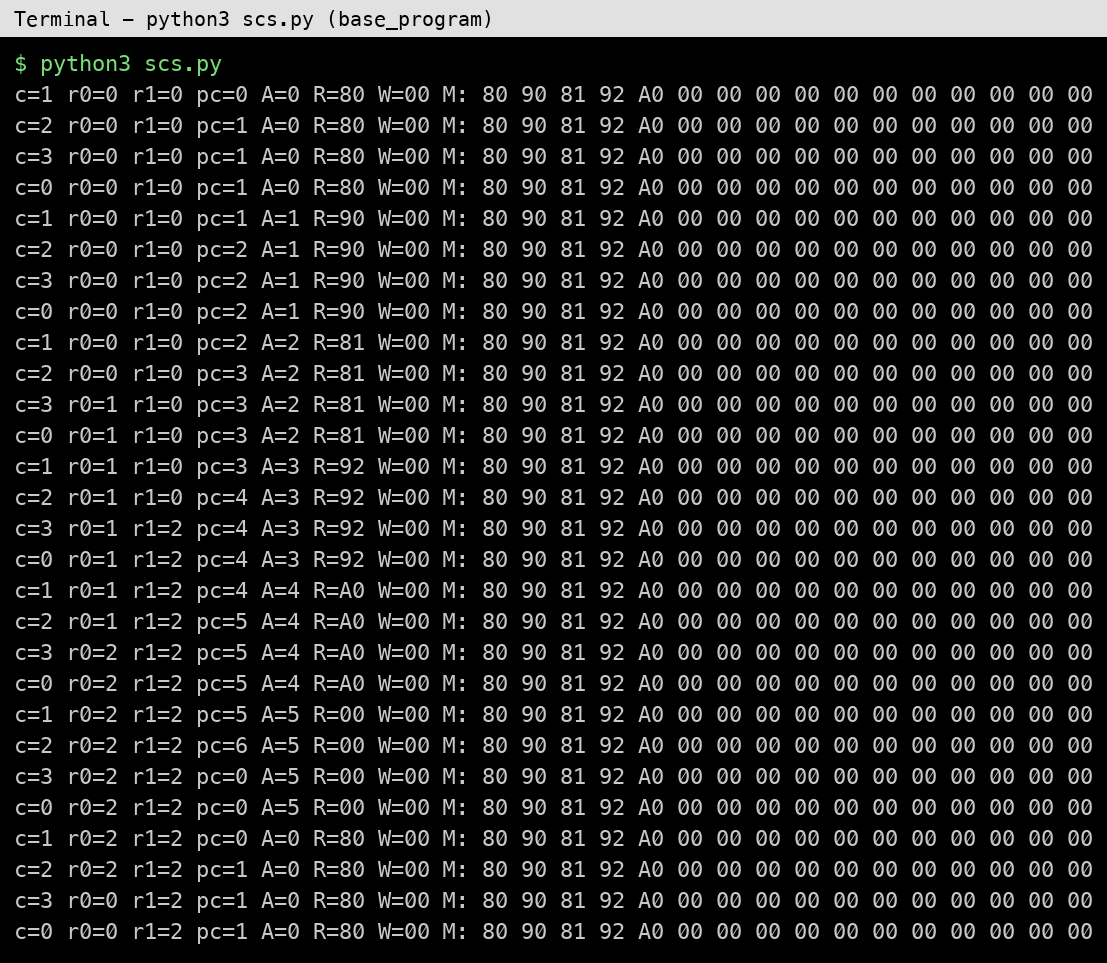
\includegraphics[width=0.85\textwidth]{img/py_1_base.png}
    \caption{Przebieg programu bazowego \kod{scs.py}}
    \label{fig:py1}
\end{figure}

Każda linia opisuje stan po jednym takcie zegara:
\begin{itemize}
    \item \kod{c} - numer stanu w cyklu instrukcji (0\ldots3),
    \item \kod{r0}, \kod{r1}, \kod{pc} -- zawartość rejestrów,
    \item \kod{A} - adres na magistrali adresowej pamięci,
    \item \kod{R} - dane na magistrali odczytu (pamięć $\rightarrow$ procesor),
    \item \kod{W} - dane na magistrali zapisu (procesor $\rightarrow$ pamięć),
    \item \kod{M} - zawartość wszystkich 16 komórek pamięci.
\end{itemize}

Na Rysunku \ref{fig:py1} widać, co dzieje się w kolejnych stanach. W linii \kod{c=1}
procesor wystawia na magistralę adres instrukcji (\kod{A=pc}), następnie w linii \kod{c=2}
kod instrukcji trafia do rejestru \kod{opcode}, a \kod{pc} zwiększa się o~1. W linii
\kod{c=3} instrukcja jest wykonywana: np. dla \kod{81} rejestr \kod{r0} zmienia się
z~0 na~1, a dla \kod{92} \kod{r1} przyjmuje wartość~2. Po instrukcji \kod{A0} oba
rejestry są równe~2. Instrukcja \kod{00} (\kod{jmp \#0}) w stanie \kod{c=3} wpisuje
do licznika \kod{pc=0}, dlatego w następnym cyklu procesor ponownie pobiera
instrukcję spod adresu 0 i program się zapętla.

\bigskip
Sposób kodowania instrukcji przedstawia drzewo dekodera z dokumentacji rdzenia
(Rysunek \ref{fig:dekoder}). Na jego podstawie można scharakteryzować możliwości
procesora w bazowej konfiguracji:
\begin{figure}[H]
    \centering
    \textit{Instrukcja skoku i arytmetyczna}\\[4pt]
    \instr{jmp addr}
        {\B0 & \B0 & \B0 & \B0 & \multicolumn{4}{c|}{addr}}
        {skok bezwarunkowy, PC = addr}
    \instr{add r0, r1}
        {\B0 & \B0 & \B1 & \B0 & X & X & X & X}
        {R0 = R0 + R1}
    \\[10pt]
    \textit{Instrukcje kopiowania i przesłań}\\[4pt]
    \instr{mov rn, \#imm}
        {\B1 & \B0 & \B0 & rn & \multicolumn{4}{c|}{\#imm}}
        {stała natychmiastowa $\rightarrow$ rejestr}
    \instr{mov rn, rm}
        {\B1 & \B0 & \B1 & rn & X & X & X & X}
        {rejestr $\rightarrow$ rejestr}
    \\[8pt]
    \instr{ldr rn, addr}
        {\B1 & \B1 & \B0 & rn & \multicolumn{4}{c|}{addr}}
        {pamięć $\rightarrow$ rejestr}
    \instr{str rn, addr}
        {\B1 & \B1 & \B1 & rn & \multicolumn{4}{c|}{addr}}
        {rejestr $\rightarrow$ pamięć}
    \caption{Kodowanie instrukcji mikroprocesora w bazowej konfiguracji}
    \label{fig:kodowanie}
\end{figure}

W bazowej konfiguracji procesor obsługuje trzy klasy instrukcji:
\begin{itemize}
    \item \textbf{skoki} -- wyłącznie skok bezwarunkowy pod adres bezwzględny
          (\kod{jmp addr}); brak skoków warunkowych, względnych i wywołań
          podprogramów (brak stosu i flag),
    \item \textbf{przesłania} -- stała $\rightarrow$ rejestr (\kod{mov rn, \#imm}),
          rejestr $\rightarrow$ rejestr (\kod{mov rn, rm}),
          pamięć $\rightarrow$ rejestr (\kod{ldr}) i rejestr $\rightarrow$ pamięć
          (\kod{str}); brak przesłań pamięć $\rightarrow$ pamięć,
    \item \textbf{przetwarzanie danych} -- jedna operacja: dodawanie
          \kod{add r0, r1} (R0 = R0 + R1, modulo 16); brak odejmowania,
          mnożenia, operacji logicznych i przesunięć.
\end{itemize}

Wszystkie instrukcje mają \textbf{stałą długość 8 bitów i jednolity format}
(4 bity kodu operacji, 4 bity argumentu), jest ich bardzo mało, operacje
arytmetyczne działają wyłącznie na rejestrach, a dostęp do pamięci odbywa się
tylko przez osobne instrukcje \kod{ldr}/\kod{str} (architektura
\textit{load/store}). Każda instrukcja wykonuje się w tej samej liczbie taktów.
Są to cechy architektury \textbf{RISC}. Procesor CISC miałby instrukcje o zmiennej
długości, złożone tryby adresowania i operacje arytmetyczne bezpośrednio na pamięci.

\begin{figure}[H]
    \centering
    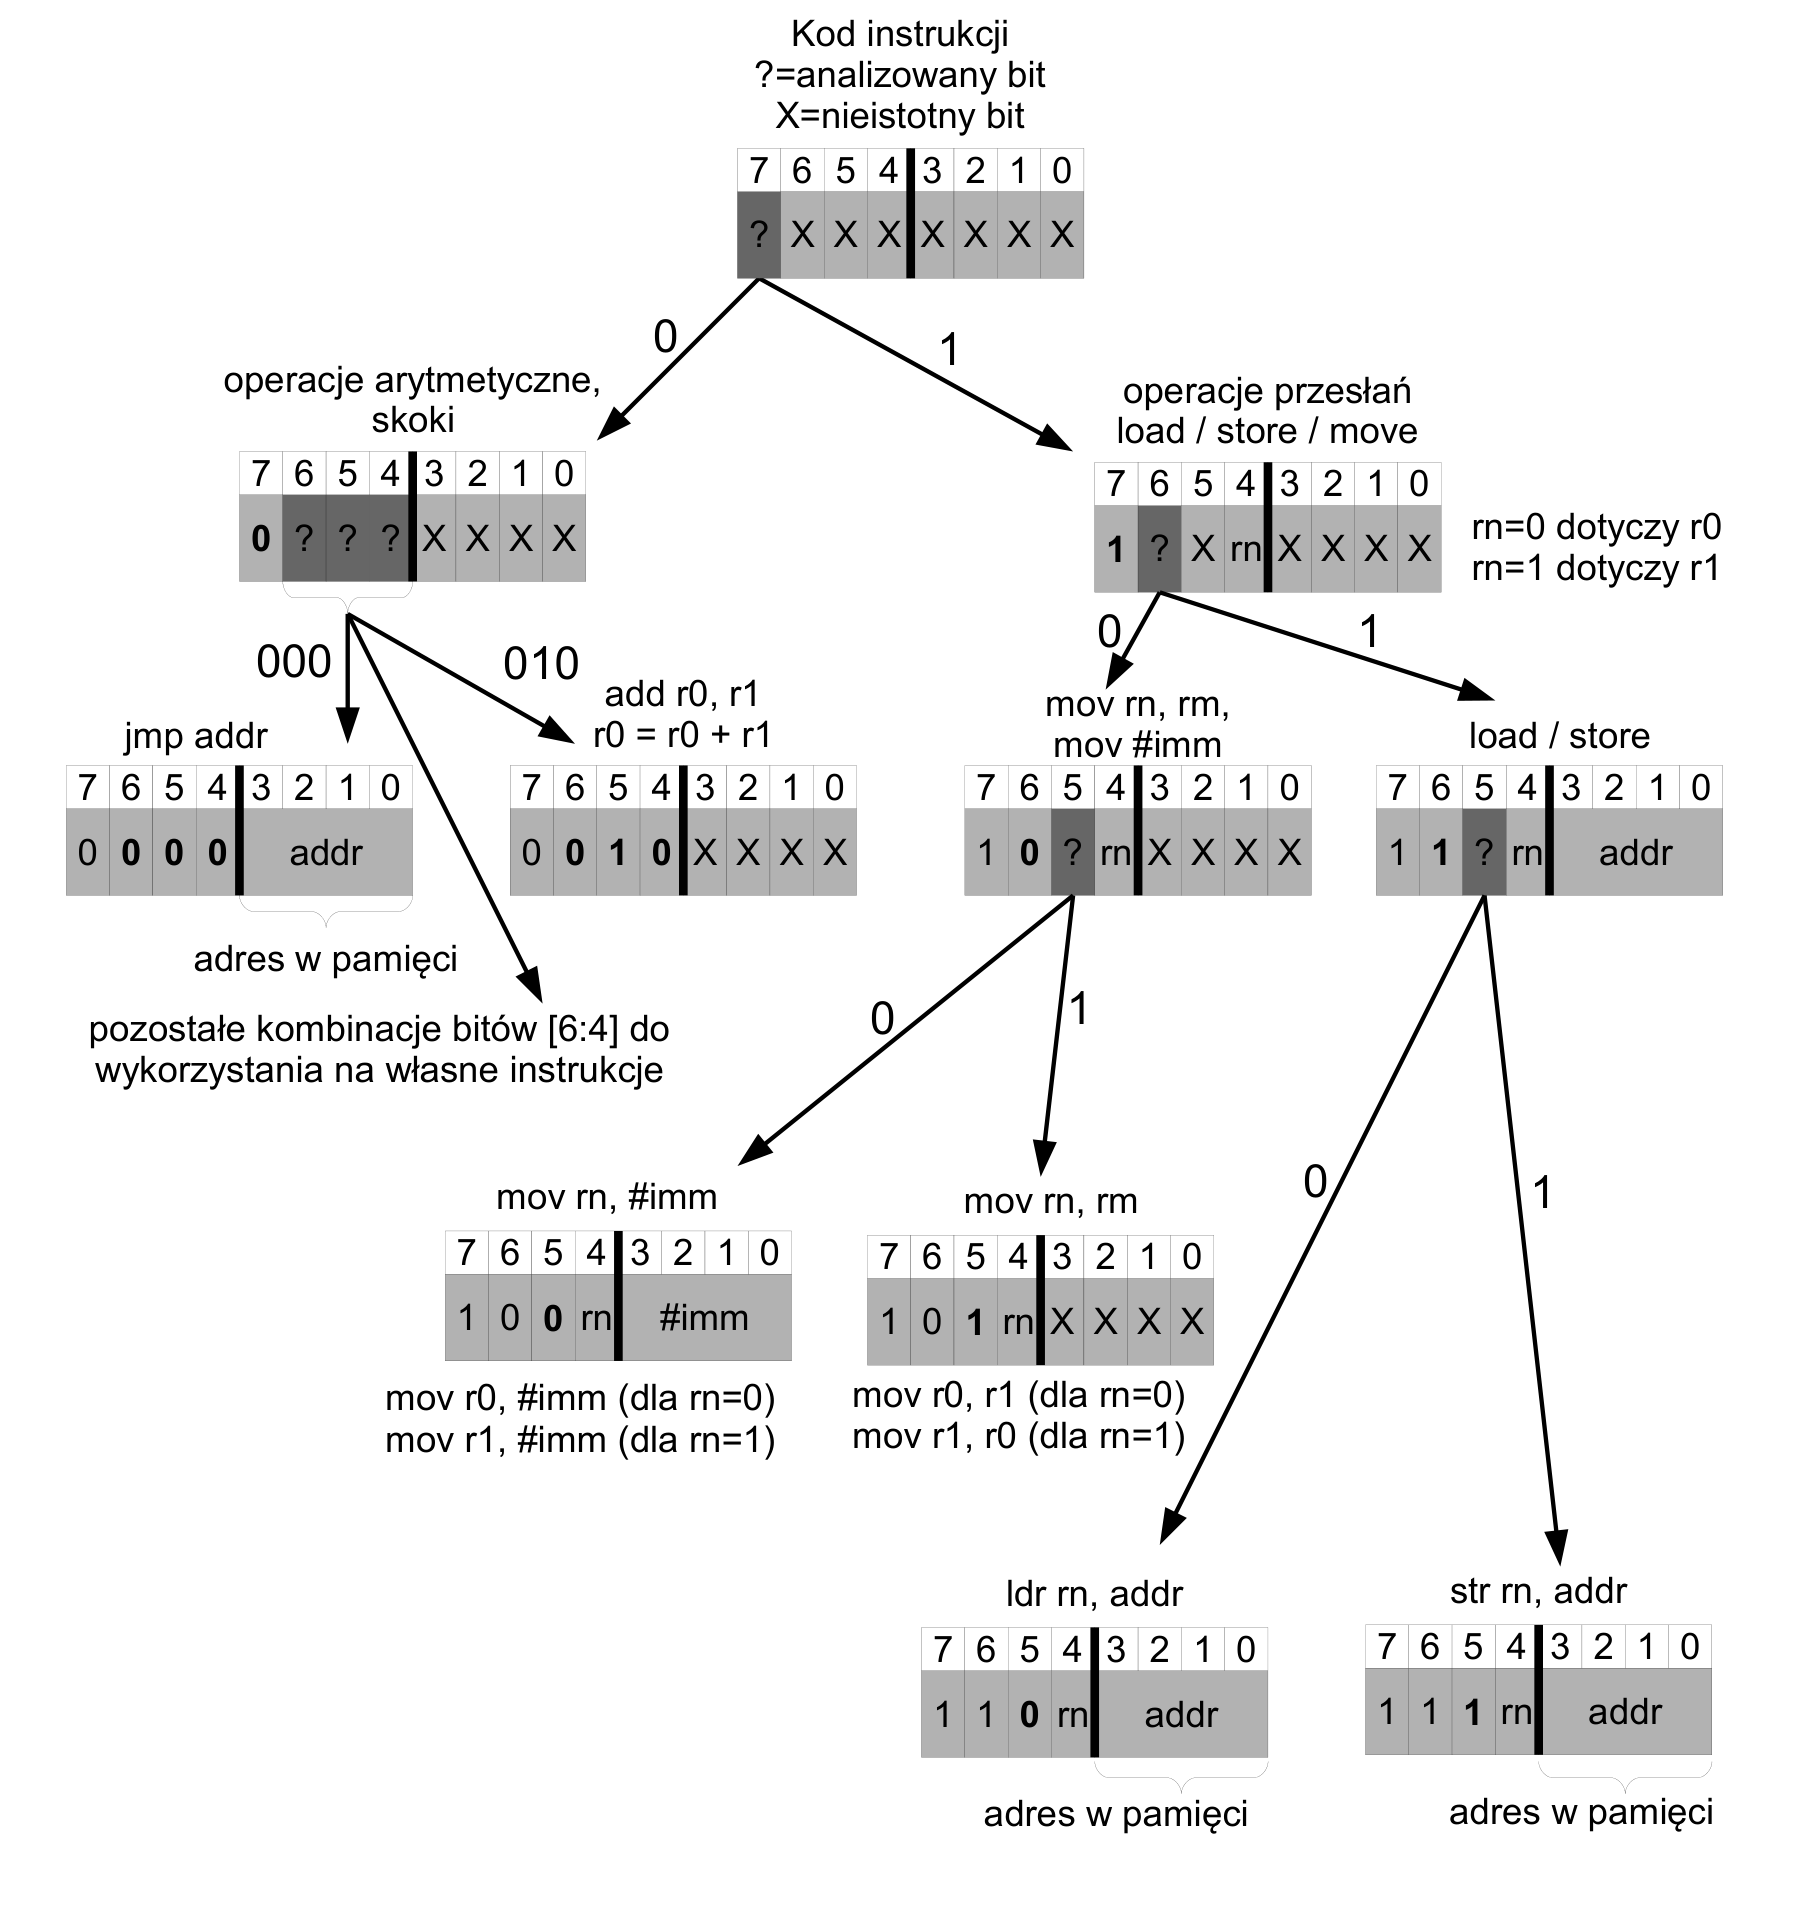
\includegraphics[width=0.75\textwidth]{img/trm_dekoder.png}
    \caption{Schemat dekodowania instrukcji mikroprocesora (źródło: \cite{trm})}
    \label{fig:dekoder}
\end{figure}

\subsection{Modyfikacja o własny program}
\label{sec:py_load_store}
Zgodnie z instrukcją listę \kod{base\_program} przemianowano na
\kod{load\_store\_program} i wpisano do niej program wykonujący kolejno:
wyzerowanie R0 i R1, wyzerowanie komórki 14, wpisanie 6 do R0, dodanie do R0
zawartości komórki 13 (dana wejściowa \kod{0x05}), zapis R0 do komórki 14
i powrót na początek (Tabela \ref{tab:ls}, Rysunek \ref{fig:nvim2}).

\begin{table}[H]
    \centering
    \begin{tabular}{|c|c|c|l|}
        \hline
        \rowcolor{gray!25} Adres & Kod & Instrukcja & Działanie \\ \hline
        00 & 80 & \kod{mov r0, \#0}  & R0 = 0 \\ \hline
        01 & 90 & \kod{mov r1, \#0}  & R1 = 0 \\ \hline
        02 & EE & \kod{str r0, 14}   & M[14] = R0 = 0 \\ \hline
        03 & 86 & \kod{mov r0, \#6}  & R0 = 6 \\ \hline
        04 & DD & \kod{ldr r1, 13}   & R1 = M[13] = 5 \\ \hline
        05 & 20 & \kod{add r0, r1}   & R0 = R0 + R1 = 0xB \\ \hline
        06 & EE & \kod{str r0, 14}   & M[14] = R0 = 0xB \\ \hline
        07 & 00 & \kod{jmp \#0}      & PC = 0 \\ \hline
        13 & 05 & -- & dana wejściowa \\ \hline
    \end{tabular}
    \caption{Program \kod{load\_store\_program}}
    \label{tab:ls}
\end{table}

Dodawanie wymaga, aby oba składniki były w rejestrach, dlatego liczba z komórki 13
jest najpierw wczytywana do R1 instrukcją \kod{ldr r1, 13}. To bezpośredni skutek
architektury \textit{load/store}.

\begin{figure}[H]
    \centering
    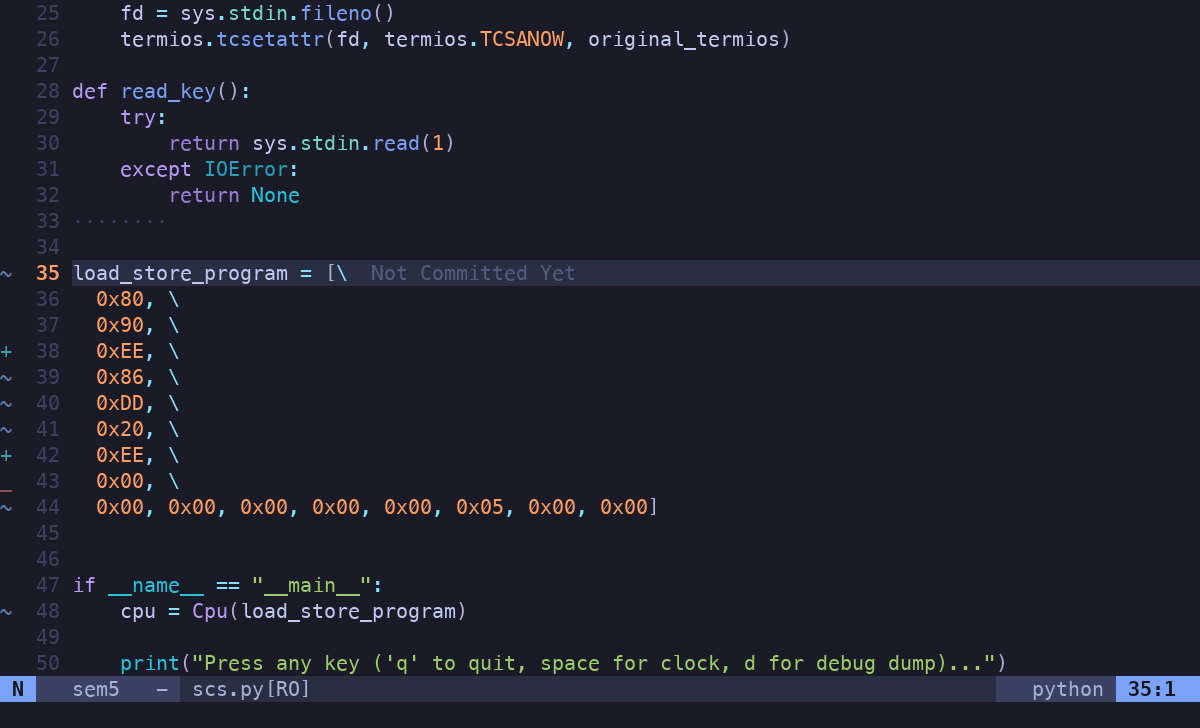
\includegraphics[width=0.8\textwidth]{img/nvim_2_load_store.png}
    \caption{Lista \kod{load\_store\_program} w pliku \kod{scs.py}}
    \label{fig:nvim2}
\end{figure}

\begin{figure}[H]
    \centering
    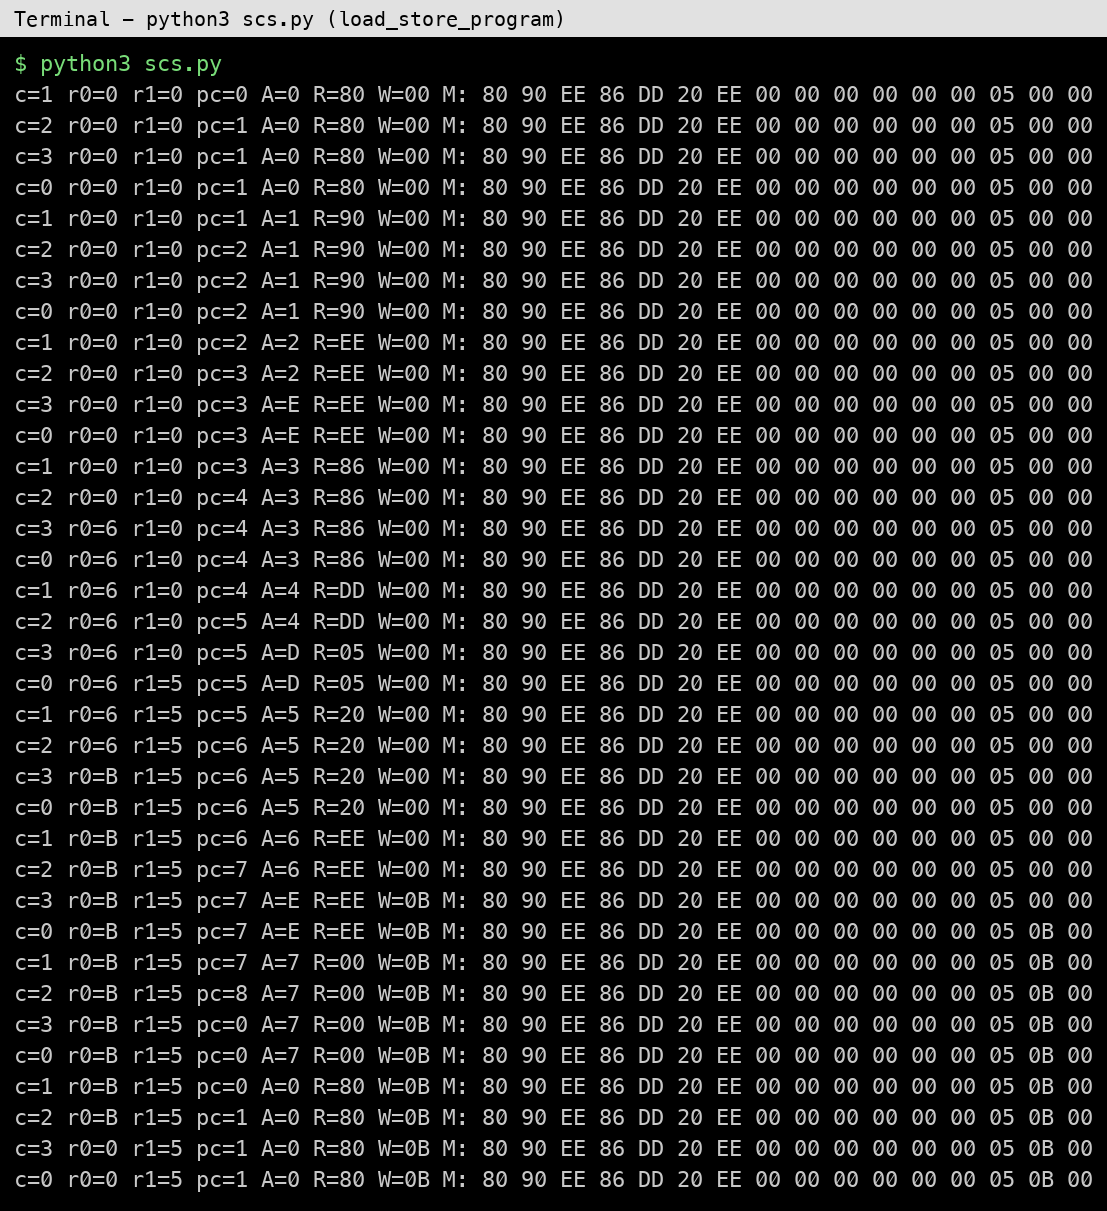
\includegraphics[width=0.85\textwidth]{img/py_2_load_store.png}
    \caption{Przebieg programu \kod{load\_store\_program} w modelu Python}
    \label{fig:py2}
\end{figure}

Na Rysunku \ref{fig:py2} widać, że po instrukcji \kod{DD} (\kod{pc=5}) rejestr
\kod{r1} przyjmuje wartość~5 odczytaną spod adresu \kod{A=D}, a po \kod{20}
\kod{r0=B} ($6+5=11$). W stanie \kod{c=3} instrukcji \kod{EE} na magistrali pojawia
się adres \kod{A=E} i dana \kod{W=0B}, a w następnej linii wartość \kod{0B}
widać już w komórce 14 zrzutu pamięci \kod{M}.

\bigskip
\textbf{Po czym poznajemy, że program się zapętlił?} Po instrukcji \kod{00}
licznik \kod{pc} wraca do 0, po czym procesor ponownie pobiera \kod{80}
(\kod{R=80}) i wykonuje dokładnie tę samą sekwencję stanów. Zawartość pamięci
w kolejnych obiegach już się nie zmienia: komórka 14 jest najpierw zerowana, a potem
znów otrzymuje \kod{0B}.

\bigskip
Zrzut \kod{M} pokazuje też, że \textbf{program i dane leżą w tej samej pamięci}:
kody instrukcji zajmują komórki 0--7, a dane komórki 13 i 14. Procesor korzysta
z jednej przestrzeni adresowej i jednej magistrali zarówno do pobierania instrukcji,
jak i do odczytu i zapisu danych. Jest to więc \textbf{architektura von Neumanna},
a nie harwardzka (ta ma osobne pamięci i magistrale dla programu i dla danych).

\subsection{Obsługa niezdefiniowanej instrukcji}
\label{sec:py_callback}
Bazowa klasa \kod{Cpu} ignorowała kody, których nie znała. W tym kroku do
konstruktora dodano opcjonalny argument \kod{undefined\_cb} -- funkcję wywoływaną
z adresem nieznanej instrukcji (Rysunek \ref{fig:nvim3a}). Dekoder w stanie 2 otrzymał
gałąź \kod{else}, do której trafiają wszystkie nieobsługiwane kody
(Rysunek \ref{fig:nvim3b}). W \kod{scs.py} zdefiniowano funkcję \kod{undefined()},
przekazywaną do konstruktora, oraz drugi program \kod{program\_2\_load\_store}
używający instrukcji \kod{0x30} i \kod{0x40}, których procesor jeszcze nie zna
(Rysunek \ref{fig:nvim3c}, Tabela \ref{tab:p2}).

\begin{figure}[H]
    \centering
    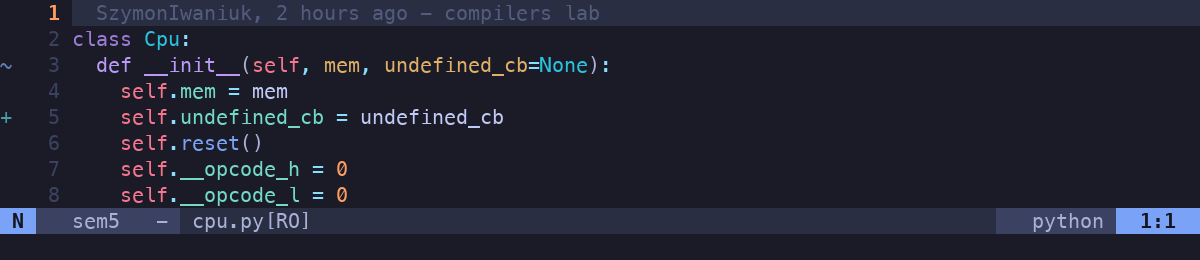
\includegraphics[width=0.8\textwidth]{img/nvim_3_cpu_init.png}
    \caption{Konstruktor klasy \kod{Cpu} z argumentem \kod{undefined\_cb} (\kod{cpu.py})}
    \label{fig:nvim3a}
\end{figure}

\begin{figure}[H]
    \centering
    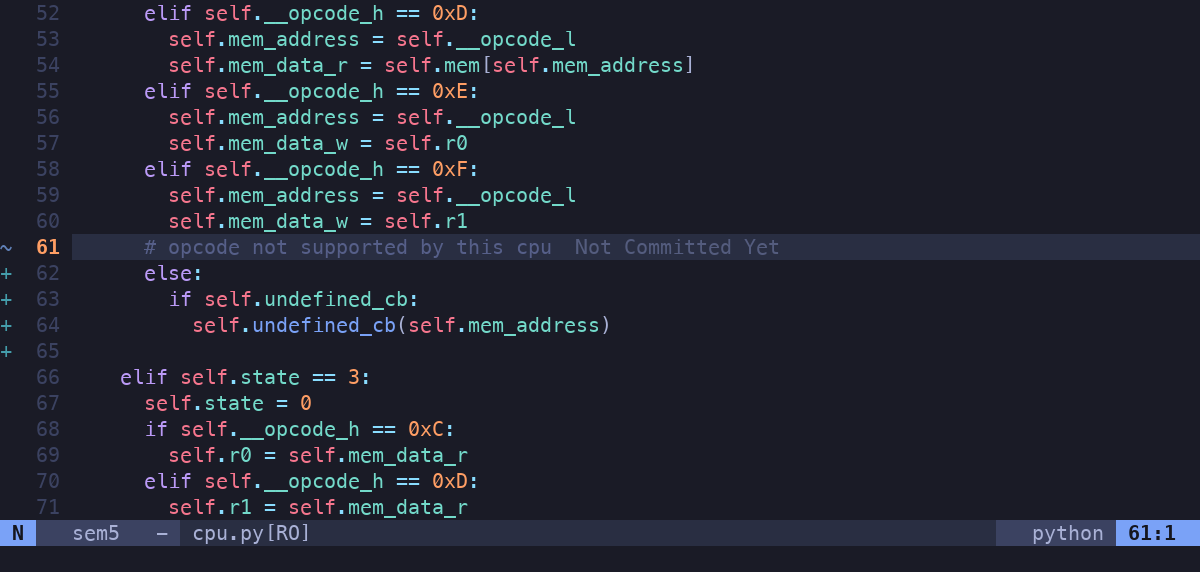
\includegraphics[width=0.8\textwidth]{img/nvim_3_cpu_callback.png}
    \caption{Wykrywanie nieobsługiwanych kodów w stanie 2 (\kod{cpu.py})}
    \label{fig:nvim3b}
\end{figure}

\begin{figure}[H]
    \centering
    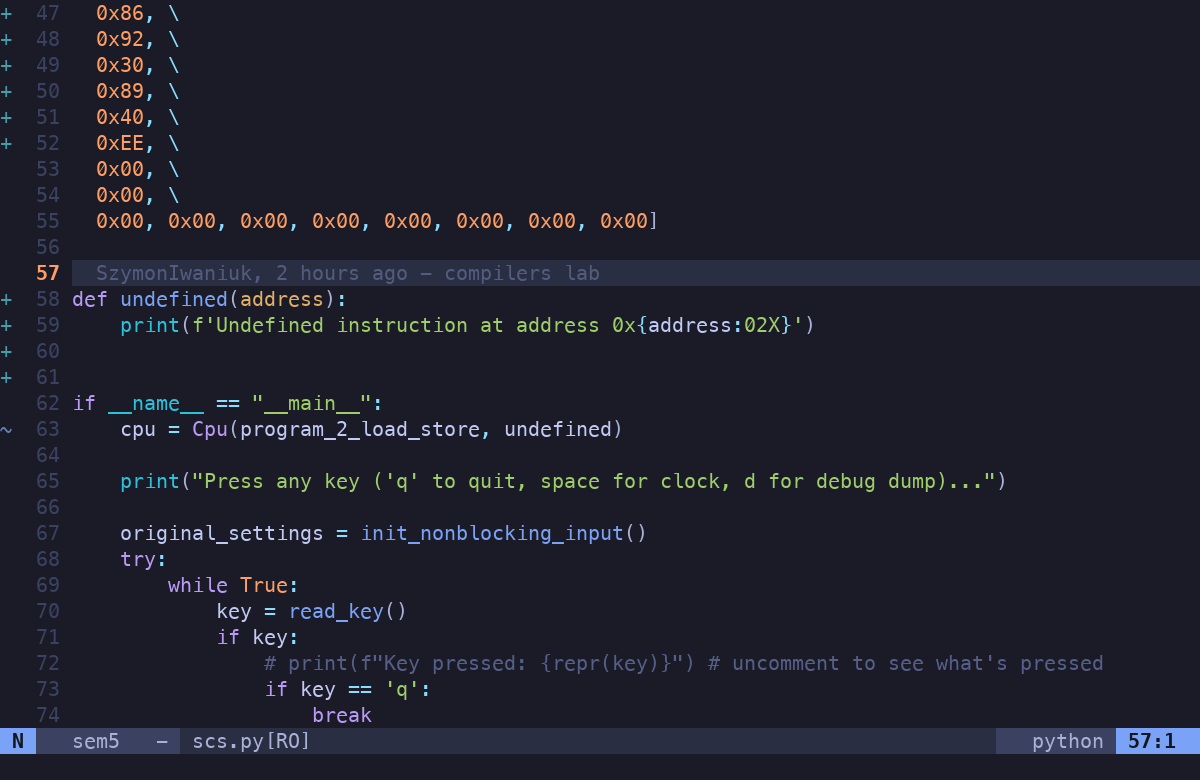
\includegraphics[width=0.8\textwidth]{img/nvim_3_scs_callback.png}
    \caption{Program \kod{program\_2\_load\_store} i funkcja \kod{undefined()} (\kod{scs.py})}
    \label{fig:nvim3c}
\end{figure}

\begin{table}[H]
    \centering
    \begin{tabular}{|c|c|c|l|}
        \hline
        \rowcolor{gray!25} Adres & Kod & Instrukcja & Działanie \\ \hline
        00 & 86 & \kod{mov r0, \#6} & R0 = 6 \\ \hline
        01 & 92 & \kod{mov r1, \#2} & R1 = 2 \\ \hline
        02 & 30 & \kod{add r1, r0}  & R1 = R0 + R1 \quad (nowa) \\ \hline
        03 & 89 & \kod{mov r0, \#9} & R0 = 9 \\ \hline
        04 & 40 & \kod{sub r0, r1}  & R0 = R0 $-$ R1 \quad (nowa) \\ \hline
        05 & EE & \kod{str r0, 14}  & M[14] = R0 \\ \hline
        06 & 00 & \kod{jmp \#0}     & PC = 0 \\ \hline
    \end{tabular}
    \caption{Program \kod{program\_2\_load\_store}}
    \label{tab:p2}
\end{table}

\begin{figure}[H]
    \centering
    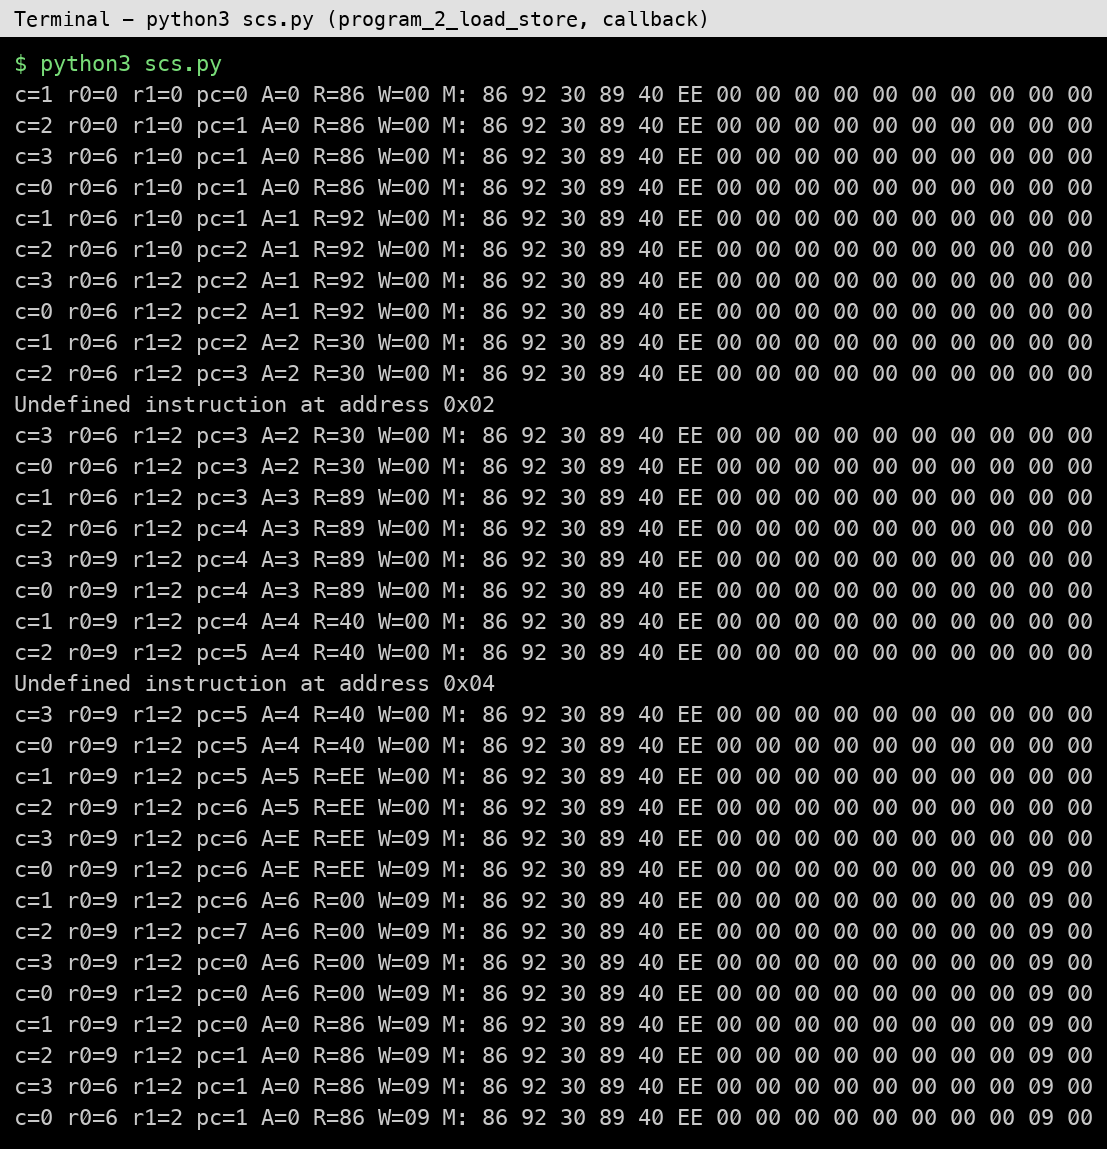
\includegraphics[width=0.85\textwidth]{img/py_3_callback.png}
    \caption{Przebieg \kod{program\_2\_load\_store} przed implementacją nowych instrukcji}
    \label{fig:py3}
\end{figure}

Na Rysunku \ref{fig:py3} po zdekodowaniu \kod{30} (adres 2) i \kod{40} (adres 4)
pojawiają się komunikaty \kod{Undefined instruction at address 0x02} oraz
\kod{0x04}. Ponieważ procesor tych kodów nie zna, nie zmieniają one rejestrów:
po \kod{30} \kod{r1} nadal ma wartość 2, a po \kod{40} \kod{r0} nadal wynosi 9.
Dlatego \kod{EE} zapisuje do komórki 14 wartość \kod{09}.

\subsection{Dodanie nowych instrukcji}
\label{sec:py_new}
Następnie dodano nowe instrukcje w taki sam sposób, w jaki zrealizowano je w module \kod{cpu.py}
(Rysunek \ref{fig:nvim4}, Tabela \ref{tab:nowe}).
Bit 4 kodu operacji wybiera rejestr, do którego trafia wynik, a dla
odejmowania wykorzystano wolną kombinację bitów [6:4] = 10x. Funkcja zwrotna
pozostała w kodzie i nadal wykrywa kody, które pozostały nieobsługiwane (np. \kod{0x10},
\kod{0x60}, \kod{0x70}).

\begin{table}[H]
    \centering
    \begin{tabular}{|c|c|c|l|}
        \hline
        \rowcolor{gray!25} Kod & Bity 7..4 & Instrukcja & Działanie \\ \hline
        \kod{2X} & 0010 & \kod{add r0, r1} & R0 = R0 + R1 \quad (bazowa) \\ \hline
        \kod{3X} & 0011 & \kod{add r1, r0} & R1 = R0 + R1 \\ \hline
        \kod{4X} & 0100 & \kod{sub r0, r1} & R0 = R0 $-$ R1 \\ \hline
        \kod{5X} & 0101 & \kod{sub r1, r0} & R1 = R0 $-$ R1 \\ \hline
    \end{tabular}
    \caption{Instrukcje arytmetyczne po rozszerzeniu (X - bity nieistotne)}
    \label{tab:nowe}
\end{table}

\begin{figure}[H]
    \centering
    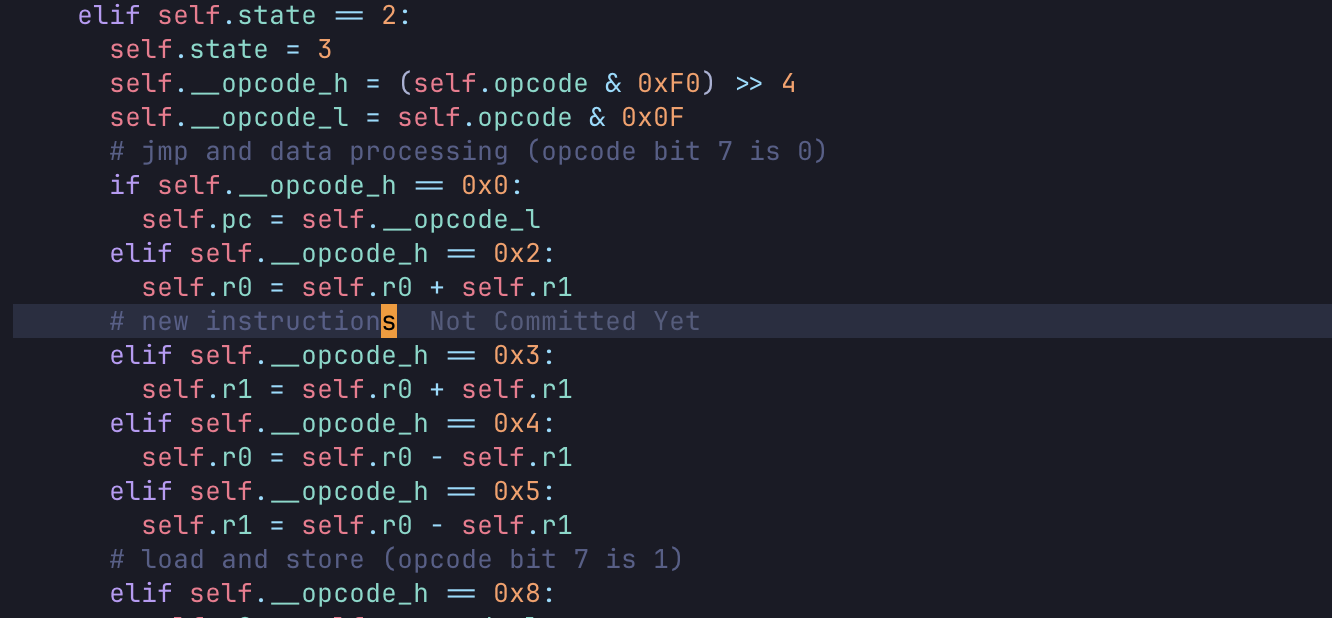
\includegraphics[width=0.8\textwidth]{img/nvim_4_cpu_instrukcje.png}
    \caption{Krok 4 -- obsługa nowych instrukcji w dekoderze (\kod{cpu.py})}
    \label{fig:nvim4}
\end{figure}

\begin{figure}[H]
    \centering
    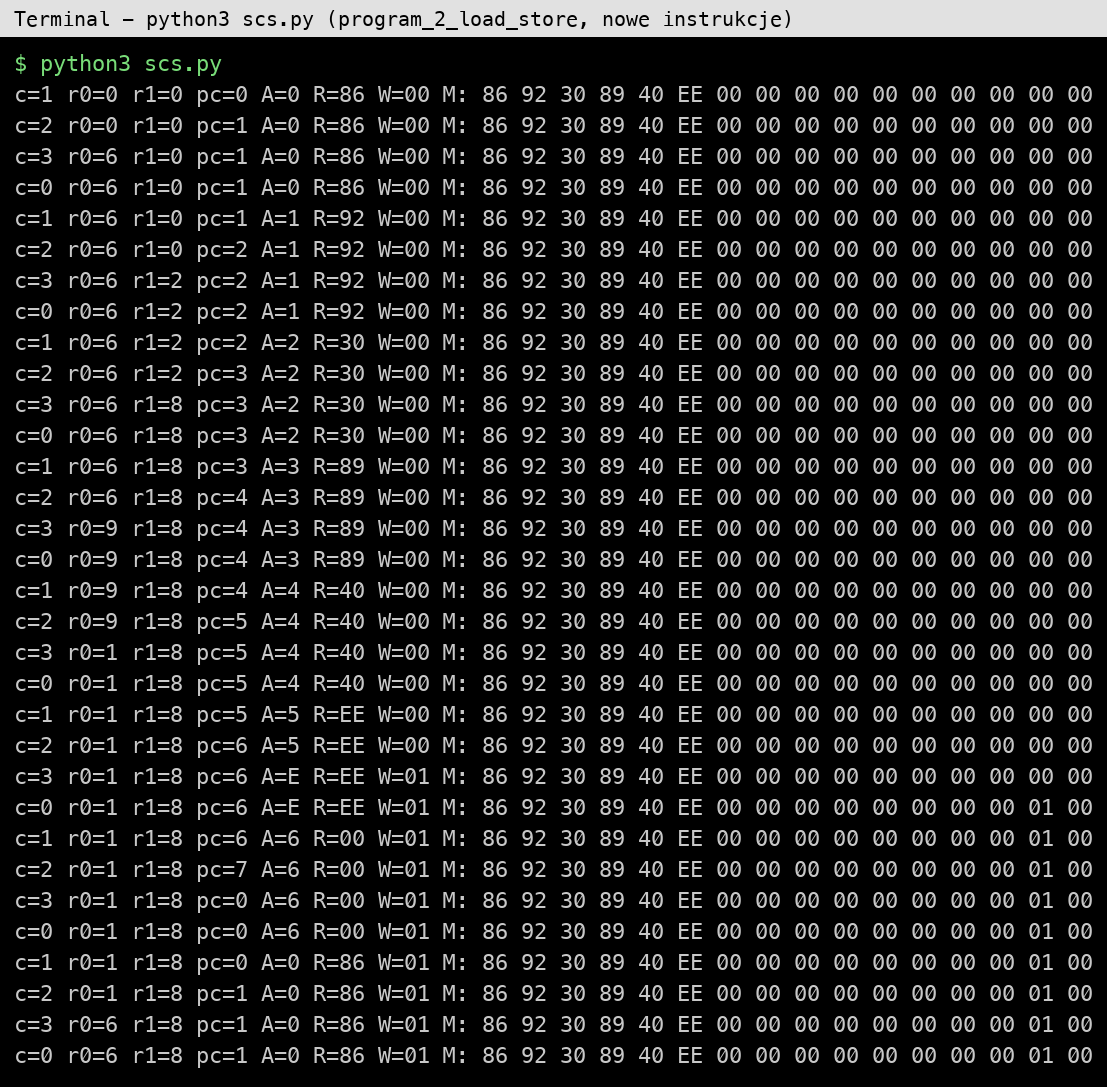
\includegraphics[width=0.85\textwidth]{img/py_4_nowe_instrukcje.png}
    \caption{Przebieg \kod{program\_2\_load\_store} po implementacji nowych instrukcji}
    \label{fig:py4}
\end{figure}

Po zmianie (Rysunek \ref{fig:py4}) komunikaty o nieznanej instrukcji zniknęły.
Instrukcja \kod{30} daje \kod{r1} = 6 + 2 = 8, następnie \kod{89} ustawia
\kod{r0=9}, a \kod{40} daje \kod{r0} = 9 $-$ 8 = 1. Instrukcja \kod{EE} zapisuje do
komórki 14 wartość \kod{01} i program się zapętla.

\paragraph{Liczby ujemne.} Rejestry mają szerokość 4 bitów, dlatego wynik
odejmowania (i dodawania) jest obcinany do 4 najmłodszych bitów -- arytmetyka
odbywa się modulo 16. Mikroprocesor nie rozróżnia liczb ze znakiem i bez znaku:
przykładowo $2 - 5$ daje wzorzec \kod{1101} (\kod{0xD}), który można interpretować
jako 13 (bez znaku) lub $-3$ (w kodzie U2, zakres $-8\ldots7$). W Pythonie takie
samo zachowanie zapewnia maska \kod{\& 0xF} (\kod{-3 \& 0xF} = 13), a w Verilogu
szerokość rejestru \kod{reg [3:0]}. Procesor nie ma flag (przeniesienia, znaku, zera)
ani skoków warunkowych, więc program nie może wykryć przekroczenia zakresu ani
zareagować na znak wyniku.

%=====================================================================
\section{Realizacja w układzie FPGA}

\subsection{System testowy}
Schemat systemu z projektu startowego przedstawia Rysunek \ref{fig:schemat}.
Rdzeń \kod{cpu1} korzysta z pamięci operacyjnej \kod{mem1},
zbudowanej z dwuportowego bloku BRAM. Port~A jest podłączony do procesora
(adres, odczyt, zapis, zezwolenie na zapis), a port~B wykorzystuje moduł
\kod{dbgu1} -- sprzętowy debugger, który po każdym takcie odczytuje stan rejestrów
(sygnały \kod{dbg\_*}) i zawartość pamięci, a następnie wysyła je przez UART
w tym samym formacie co model w Pythonie.

\begin{figure}[H]
    \centering
    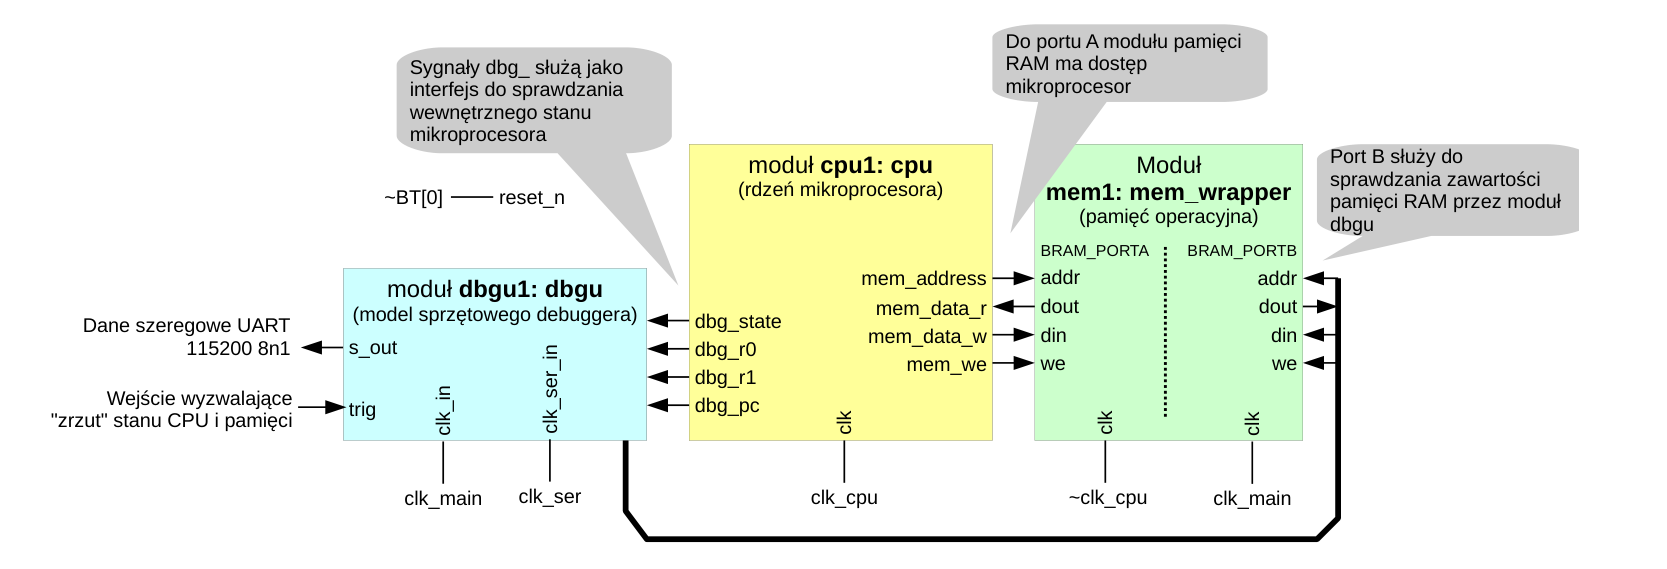
\includegraphics[width=\textwidth]{img/pdf_schemat_blokowy.png}
    \caption{Schemat blokowy systemu testowego}
    \label{fig:schemat}
\end{figure}

Tak jak w modelu, instrukcje i dane leżą w jednym bloku pamięci, do którego
procesor ma dostęp przez jeden port z jedną magistralą adresową
(\kod{mem\_address}, 4 bity, 16 komórek) -- jest to architektura von Neumanna.
Magistrale danych \kod{mem\_data\_r}/\kod{mem\_data\_w} mają 8 bitów (całe słowo
instrukcji), natomiast rejestry \kod{r0}, \kod{r1} i \kod{pc} są
4-bitowe (\kod{reg [3:0]}), a rejestr stanu 2-bitowy. Procesor jest więc
\textbf{4-bitowy} -- tyle wynosi szerokość jego jednostki arytmetycznej, rejestrów
i adresu.

Zegar procesora wybierany jest przełącznikami (Rysunek \ref{fig:zegary}).
SW[1] w dół oznacza zegar ręczny z przycisku BTN[2], a SW[1] w górę -- automatyczny
zegar 1~Hz. Przy zegarze ręcznym SW[0] w górę daje 1 impuls na naciśnięcie
(obserwacja pojedynczych \textbf{cykli zegarowych}), a SW[0] w dół -- 4 impulsy
na naciśnięcie, czyli jeden pełny \textbf{cykl instrukcji}. Ten przełącznik
odzwierciedla w sprzęcie różnicę między cyklem zegarowym a cyklem instrukcji
opisaną w części programowej.

\begin{figure}[H]
    \centering
    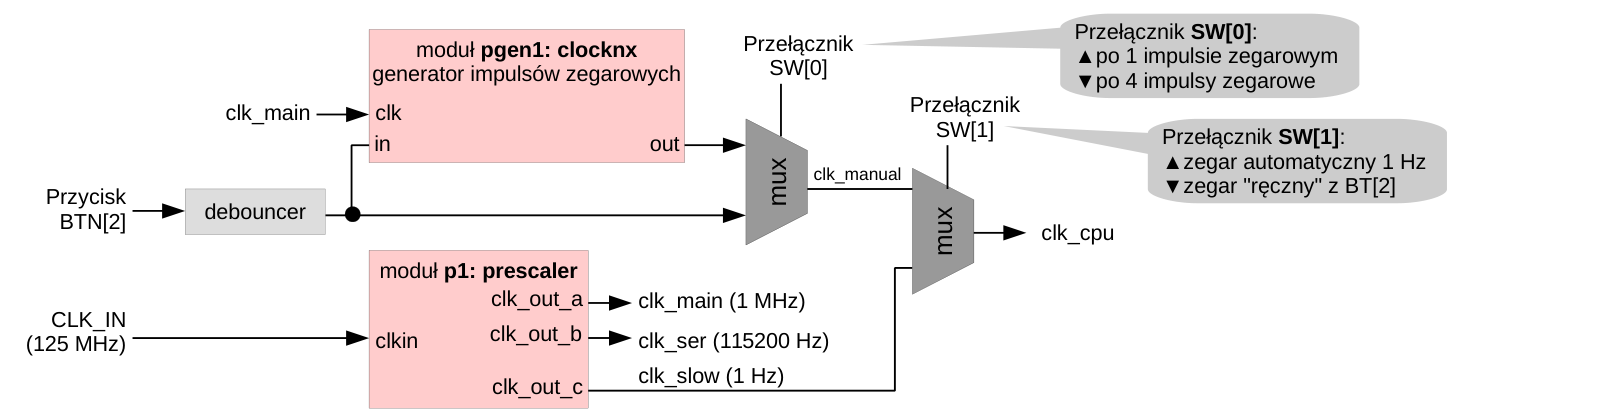
\includegraphics[width=\textwidth]{img/pdf_zegary.png}
    \caption{Podsystem dystrybucji sygnałów zegarowych}
    \label{fig:zegary}
\end{figure}

\subsection{Utworzenie systemu mikroprocesorowego w FPGA}
Projekt utworzono w Vivado 2024.1 jako \textit{RTL Project} dla płytki Zybo,
dodając pliki źródłowe z katalogu \kod{src} oraz plik ograniczeń
\kod{Constraints.xdc}. Brakujący moduł pamięci \kod{mem\_wrapper} wygenerowano
w IP Integratorze: blok \textit{Block Memory Generator} w trybie \textit{True Dual
Port RAM}, słowo 8 bitów, głębokość 16, tryb \textit{Write First}, bez rejestrów
wyjściowych, z zawartością początkową z pliku \kod{mem\_init\_start.coe}. Oba porty
wyprowadzono na zewnątrz (\textit{Make External}), utworzono \textit{HDL Wrapper},
wygenerowano bitstream i zaprogramowano układ.

\begin{figure}[H]
    \centering
    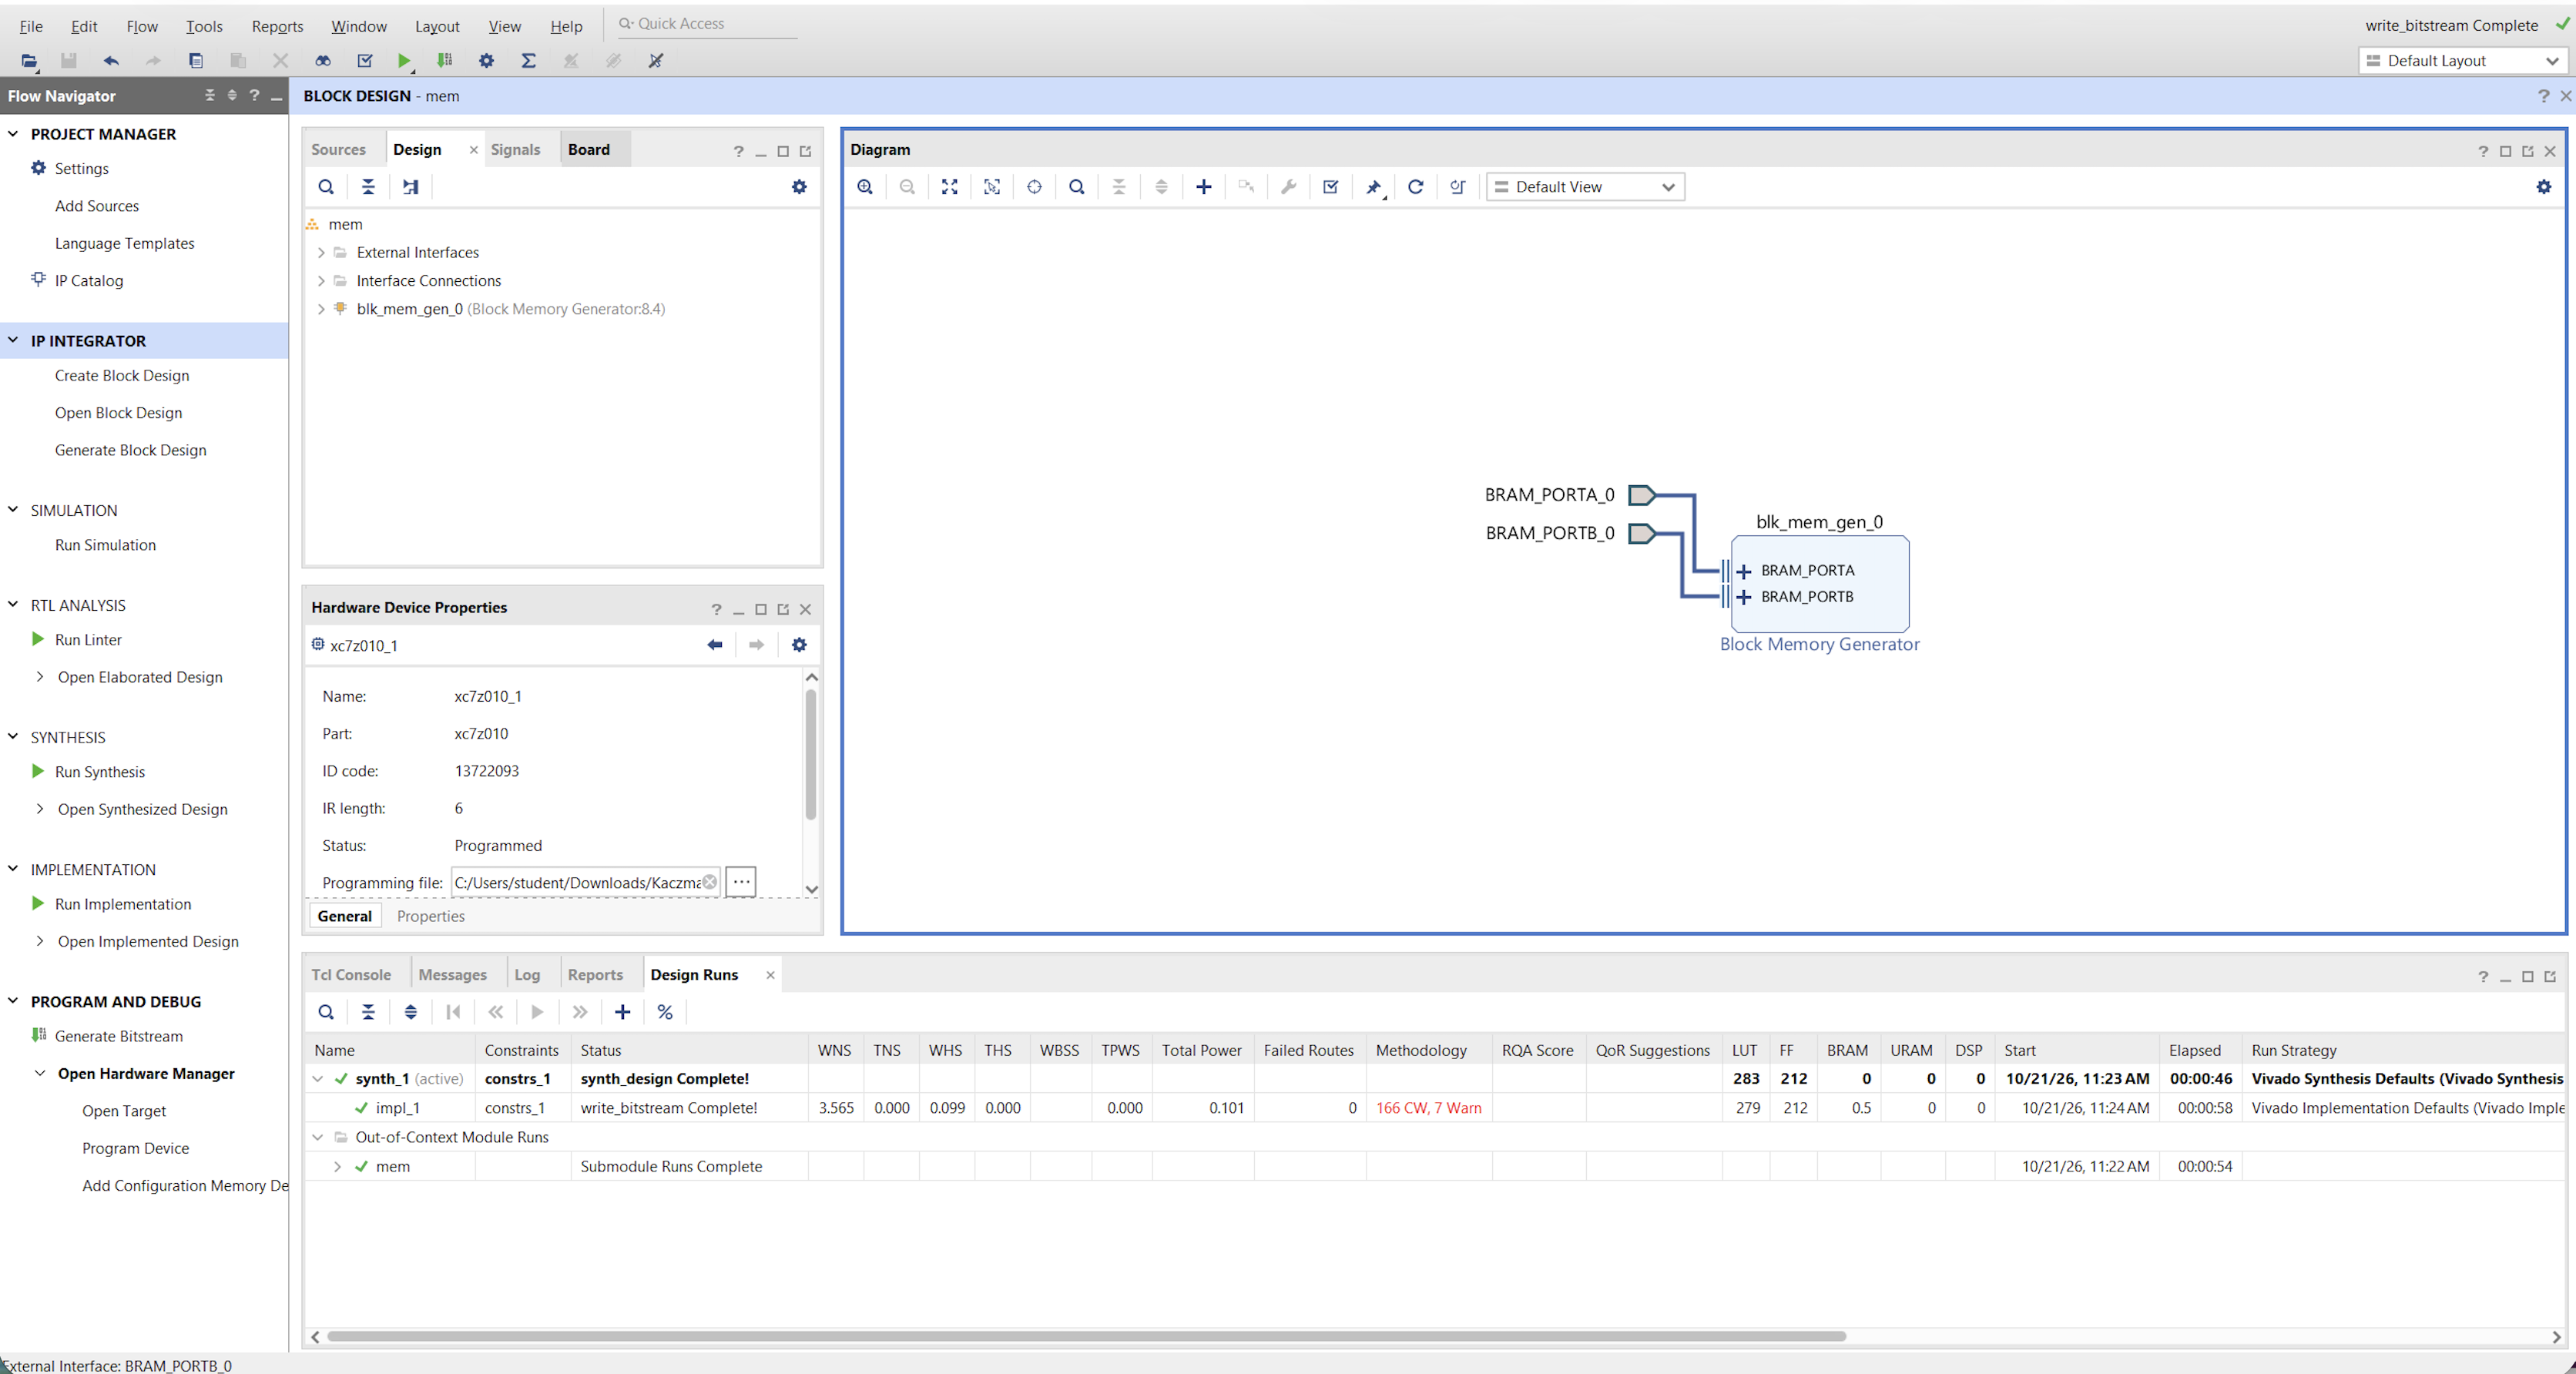
\includegraphics[width=\textwidth]{img/hw_vivado_projekt.png}
    \caption{Projekt w Vivado: block design \kod{mem}, ukończone syntezy i implementacja, układ \kod{xc7z010\_1} w stanie \textit{Programmed}}
    \label{fig:vivado}
\end{figure}

Na Rysunku \ref{fig:vivado} widać gotowy blok pamięci z wyprowadzonymi portami
\kod{BRAM\_PORTA\_0} i \kod{BRAM\_PORTB\_0}, status \kod{write\_bitstream Complete}
oraz właściwości układu \kod{xc7z010\_1} ze statusem \textit{Programmed}. Raport
implementacji pokazuje zużycie zasobów: 279 LUT, 212 przerzutników i 0,5 bloku BRAM.

\subsection{Obserwacja działania programu testowego}
Po zaprogramowaniu układu połączono się z płytką przez PuTTY, ustawiono zegar
ręczny i wyzerowano system przyciskiem BTN[0]. Kolejne naciśnięcia BTN[2] dały
przebieg programu bazowego z Tabeli \ref{tab:base} (Rysunek \ref{fig:hw1}).

\begin{figure}[H]
    \centering
    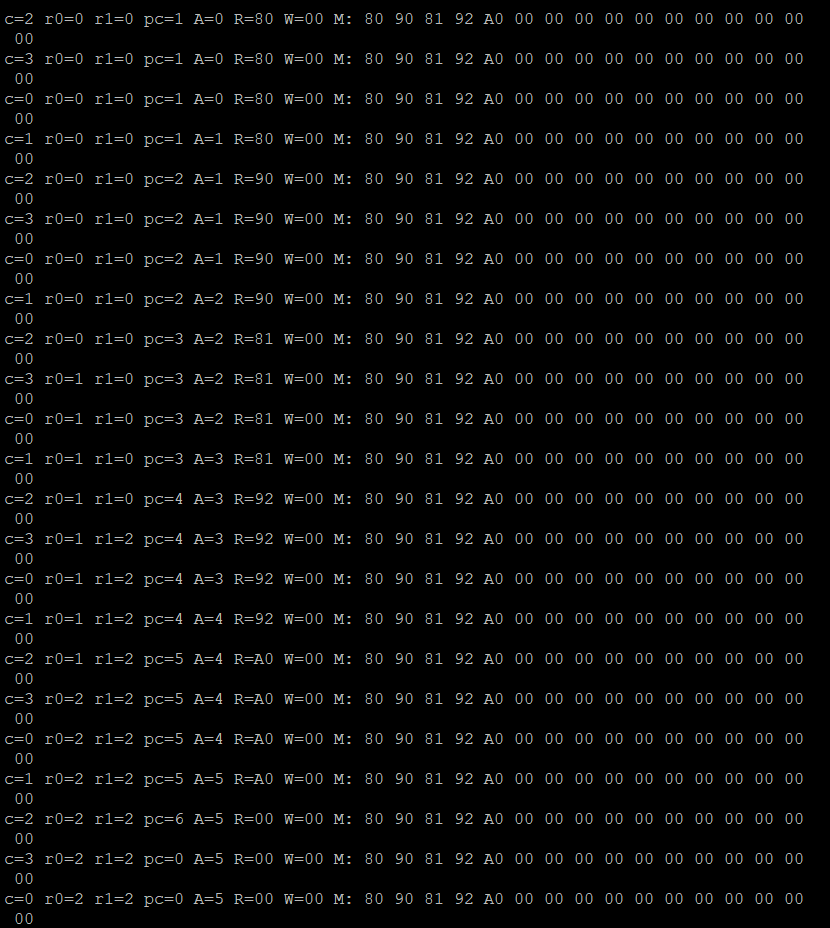
\includegraphics[width=0.8\textwidth]{img/hw_program_testowy.png}
    \caption{Program bazowy na płytce Zybo}
    \label{fig:hw1}
\end{figure}

Wartości \kod{r0}, \kod{r1} i \kod{pc} zmieniają się dokładnie tak samo jak
w modelu (Rysunek \ref{fig:py1}): po \kod{81} \kod{r0=1}, po \kod{92} \kod{r1=2},
po \kod{A0} \kod{r0=2}, a po \kod{00} \kod{pc} wraca do 0. Kod \kod{cpu.v} realizuje
cztery stany cyklu instrukcji:
\begin{enumerate}
    \setcounter{enumi}{-1}
    \item \textbf{pobranie} (\textit{instruction fetch}) -- wystawienie adresu instrukcji: \kod{mem\_address <= pc}
          (widoczne w linii \kod{c=1} jako \kod{A=pc}),
    \item \textbf{zapamiętanie kodu i inkrementacja PC} (\textit{fetch / latch}) -- \kod{opcode <= mem\_data\_r},
          \kod{pc <= pc + 1} (linia \kod{c=2}),
    \item \textbf{dekodowanie i wykonanie} (\textit{decode / execute}) -- operacja na rejestrach,
          skok lub wystawienie adresu i danej dla \kod{ldr}/\kod{str} (linia \kod{c=3}),
    \item \textbf{dostęp do pamięci / zapis wyniku} (\textit{memory access / write-back}) -- wpisanie
          odczytanej danej do rejestru (\kod{ldr}) albo ustawienie \kod{mem\_we} (\kod{str})
          (linia \kod{c=0}).
\end{enumerate}
Odpowiada to klasycznemu podziałowi na fazy \textit{fetch -- decode -- execute},
przy czym pobranie instrukcji zajmuje tu dwa takty, a dostęp do pamięci
wydzielony jest jako osobny, czwarty etap.

Procesor \textbf{nie ma potoku}: kolejna instrukcja jest pobierana dopiero po
zakończeniu poprzedniej, a każda instrukcja -- niezależnie od rodzaju -- trwa
\textbf{stałe 4 takty zegara}. Dla instrukcji, które nie korzystają
z pamięci, stan 3 nic nie robi, ale i tak zajmuje takt.

W porównaniu z modelem widać jedną różnicę: na płytce dana z pamięci (\kod{R})
pojawia się jeden takt później. Przykładowo, w linii \kod{c=1} jest już \kod{A=1},
ale nadal \kod{R=80}, a \kod{R=90} widać dopiero w linii \kod{c=2}. Wynika to
z tego, że BRAM jest pamięcią synchroniczną taktowaną zanegowanym zegarem procesora
(\kod{\textasciitilde clk\_cpu}): odczyt następuje na opadającym zboczu, czyli pół
taktu po wystawieniu adresu, już po wysłaniu linii przez debugger. Model w Pythonie
odczytuje pamięć natychmiast. Z tego samego powodu zapis danej do \kod{M} widać na
płytce o jeden takt później niż w modelu. Wartości rejestrów i ich kolejność są
identyczne.

\subsection{Implementacja własnego programu}
Program z punktu \ref{sec:py_load_store} wpisano w edytorze
plików \kod{.coe} w ustawieniach bloku pamięci, ponownie wygenerowano bitstream
i zaprogramowano układ. Początek jego przebiegu na płytce przedstawia
Rysunek \ref{fig:hw2}. W zrzucie pamięci widać kod programu
\kod{80 90 EE 86 DD 20 EE} oraz daną wejściową \kod{05} w komórce 13, a pierwsze
instrukcje wykonują się tak samo jak w modelu w Pythonie.

\begin{figure}[H]
    \centering
    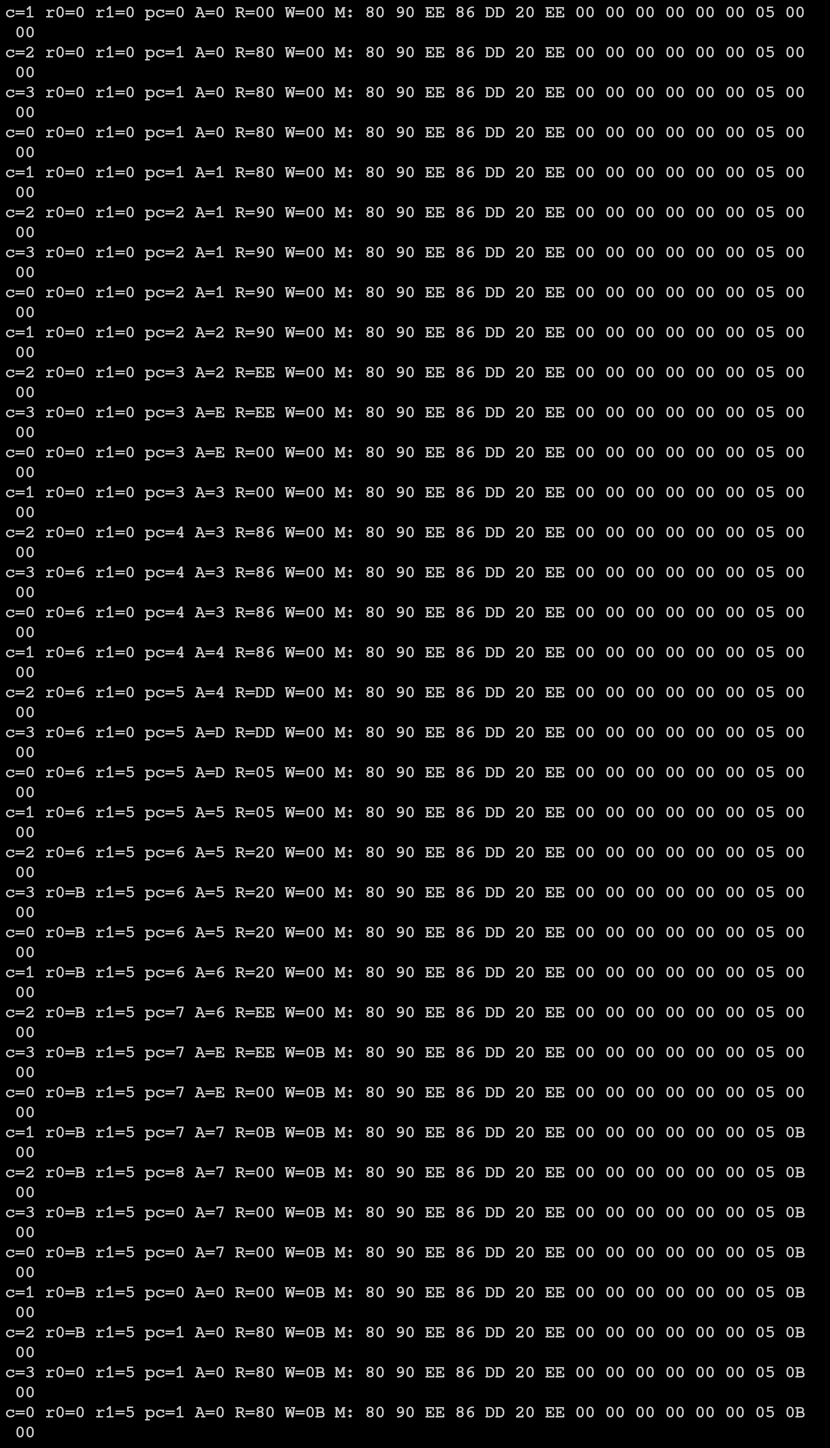
\includegraphics[width=0.75\textwidth]{img/hw_wlasny_program.png}
    \caption{Własny program na płytce Zybo}
    \label{fig:hw2}
\end{figure}

Na Rysunku \ref{fig:hw2} widać pełny obieg programu. Po instrukcji \kod{DD}
rejestr \kod{r1} przyjmuje wartość~5 odczytaną z komórki 13, po \kod{20}
\kod{r0=B} ($6+5=11$), a instrukcja \kod{EE} zapisuje \kod{0B} do komórki 14.
Następnie \kod{jmp \#0} przywraca \kod{pc=0} i program się zapętla.
Sekwencja wartości rejestrów jest identyczna jak w modelu w Pythonie,
różni się jedynie opóźnieniem magistrali \kod{R} i momentem pojawienia się zapisu
w \kod{M}, wynikającym z synchronicznej pamięci BRAM.

\subsection{Utworzenie nowej instrukcji mikroprocesora}
W pliku \kod{cpu.v} rozszerzono dekoder instrukcji arytmetycznych
(Rysunek \ref{fig:cpuv}). Kombinacje bitów [6:4] = 010 i 011 obsługują dodawanie,
przy czym bit 4 wybiera rejestr wyniku. Kombinacje 100 i 101 obsługują w ten sam
sposób nowe odejmowanie.

\begin{figure}[H]
    \centering
    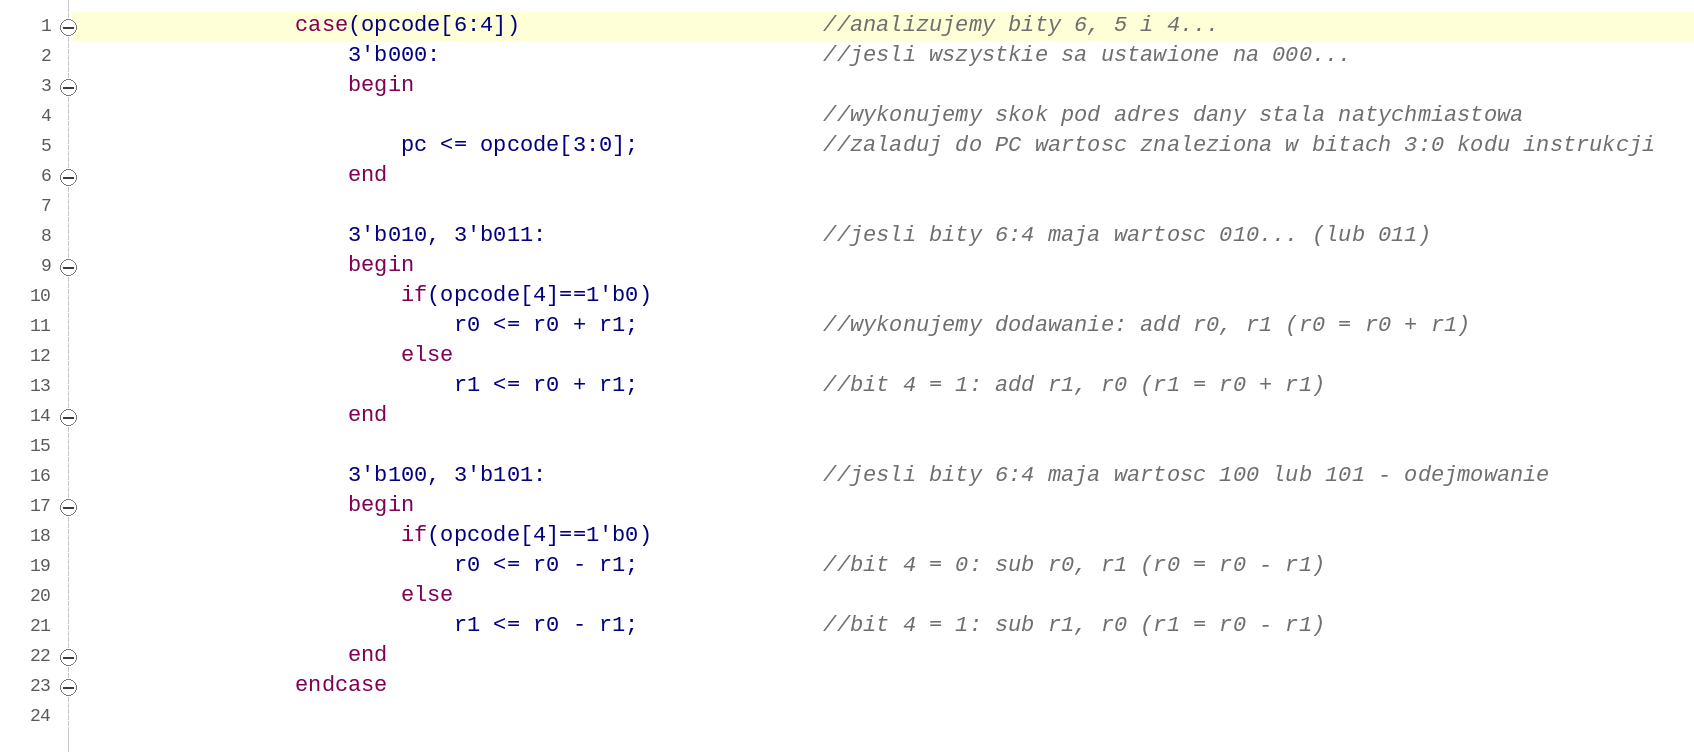
\includegraphics[width=0.85\textwidth]{img/hw_cpu_v_zmiany.png}
    \caption{Rozszerzony dekoder w pliku \kod{cpu.v}}
    \label{fig:cpuv}
\end{figure}

Do pamięci wpisano ten sam program
(\kod{86 92 30 89 40 EE 00}). Plik \kod{mem\_init\_start.coe}, z
którego Vivado inicjalizuje blok BRAM, przedstawia
Rysunek \ref{fig:coe}. Każda z 16 liczb szesnastkowych w
\kod{memory\_initialization\_vector} to zawartość kolejnej komórki pamięci,
czyli dokładnie ta sama lista co \kod{program\_2\_load\_store} w \kod{scs.py}.
Przebieg zarejestrowany na płytce przedstawia Rysunek \ref{fig:hw3}.

\begin{figure}[H]
    \centering
    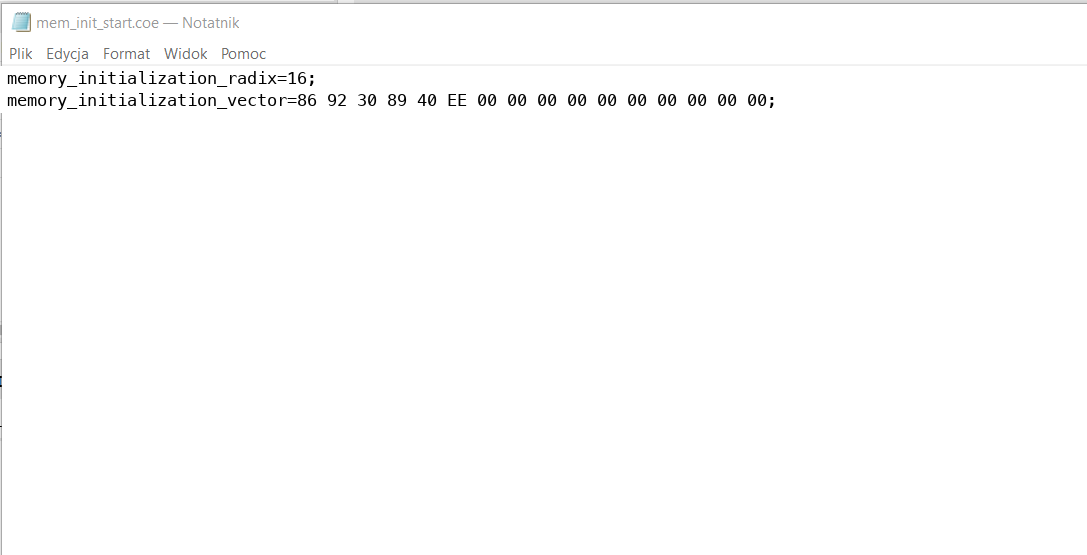
\includegraphics[width=0.8\textwidth]{img/hw_coe_nowe_instrukcje.png}
    \caption{Plik \kod{mem\_init\_start.coe} z zawartością początkową pamięci}
    \label{fig:coe}
\end{figure}

\begin{figure}[H]
    \centering
    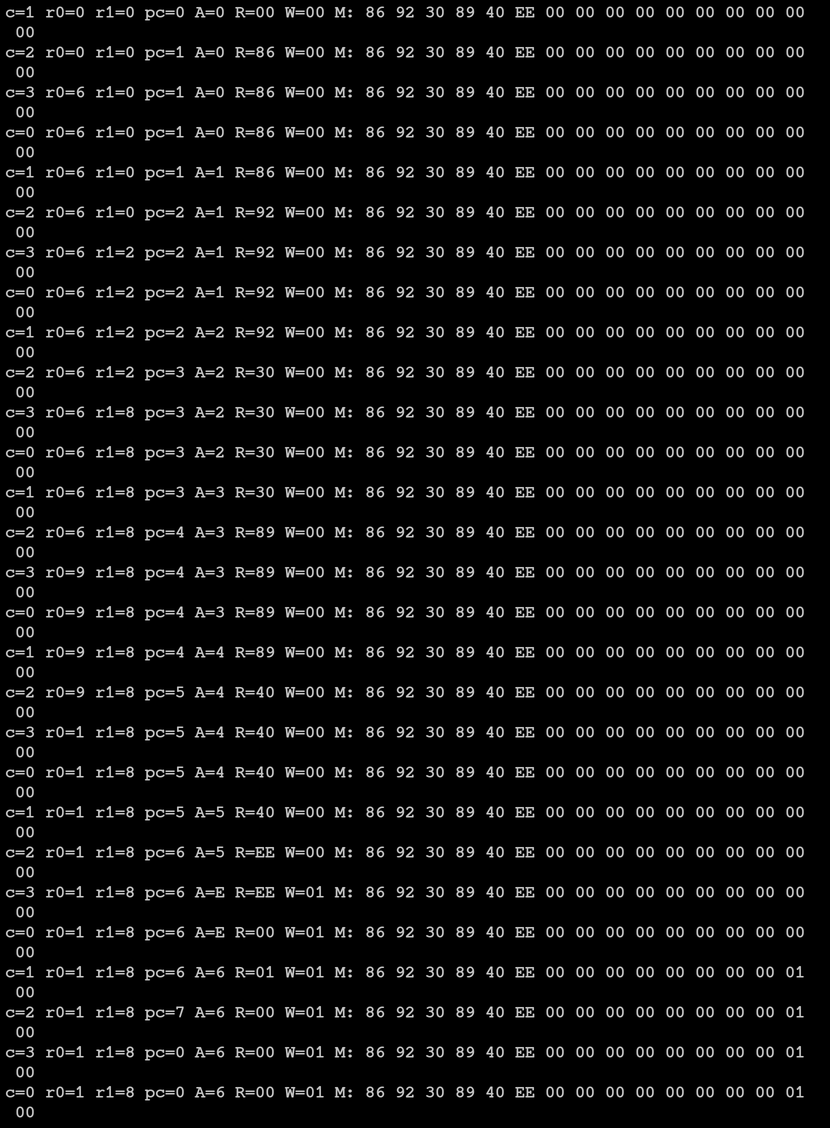
\includegraphics[width=0.85\textwidth]{img/hw_nowe_instrukcje.png}
    \caption{Program z nowymi instrukcjami na płytce Zybo}
    \label{fig:hw3}
\end{figure}

Na płytce nowe instrukcje działają zgodnie z oczekiwaniami. Po \kod{30}
rejestr \kod{r1} przyjmuje wartość $6+2=8$, następnie \kod{89} ustawia
\kod{r0=9}, a po \kod{40} \kod{r0} = $9-8=1$. Instrukcja \kod{EE}
zapisuje \kod{01} do komórki 14, a \kod{jmp \#0} zapętla program.
Przebieg jest identyczny jak w modelu w Pythonie po dodaniu nowych
instrukcji (Rysunek \ref{fig:py4}).


%=====================================================================
\section{Wnioski}
\begin{itemize}
    \item Dydaktyczny mikroprocesor SCS to 4-bitowy procesor o architekturze von
          Neumanna i cechach RISC (stały 8-bitowy format instrukcji, architektura
          load/store), z dwoma rejestrami ogólnego przeznaczenia, licznikiem programu
          i stałym czasem wykonania instrukcji równym 4 taktom, bez przetwarzania
          potokowego.
    \item Model w Pythonie i rdzeń w Verilogu mają ten sam model programowy:
          te same programy dają te same sekwencje wartości rejestrów. Różnią się
          jedynie opóźnieniem odczytu z synchronicznej pamięci BRAM.
    \item Wykrywanie nieobsługiwanych instrukcji przez funkcję zwrotną
          pozwoliło szybko sprawdzić, które kody procesor ignoruje, i
          potwierdzić, że po rozszerzeniu dekodera kody \kod{30} i \kod{40}
          są obsługiwane.
    \item Rozszerzenie dekodera o dodawanie z wyborem rejestru wyniku (bit 4)
          i o odejmowanie wymagało tylko wykorzystania wolnych kombinacji bitów
          [6:4]. Brak flag i skoków warunkowych sprawia jednak, że procesor nie
          rozróżnia liczb ujemnych ani nie wykrywa przepełnienia.
\end{itemize}

\begin{thebibliography}{9}
    \bibitem{trm} A. Brzoza, \textit{Dydaktyczny Mikroprocesor -- dokumentacja techniczna
        rdzenia mikroprocesora systemu SCS}
    \bibitem{zybo} Digilent, \textit{Zybo Reference Manual},
        \url{https://reference.digilentinc.com/reference/programmable-logic/zybo/reference-manual}.
\end{thebibliography}

\end{document}
